%%
%% This is file `sample-sigconf-authordraft.tex',
%% generated with the docstrip utility.
%%
%% The original source files were:
%%
%% samples.dtx  (with options: `all,proceedings,bibtex,authordraft')
%% 
%% IMPORTANT NOTICE:
%% 
%% For the copyright see the source file.
%% 
%% Any modified versions of this file must be renamed
%% with new filenames distinct from sample-sigconf-authordraft.tex.
%% 
%% For distribution of the original source see the terms
%% for copying and modification in the file samples.dtx.
%% 
%% This generated file may be distributed as long as the
%% original source files, as listed above, are part of the
%% same distribution. (The sources need not necessarily be
%% in the same archive or directory.)
%%
%%
%% Commands for TeXCount
%TC:macro \cite [option:text,text]
%TC:macro \citep [option:text,text]
%TC:macro \citet [option:text,text]
%TC:envir table 0 1
%TC:envir table* 0 1
%TC:envir tabular [ignore] word
%TC:envir displaymath 0 word
%TC:envir math 0 word
%TC:envir comment 0 0
%%
%% The first command in your LaTeX source must be the \documentclass
%% command.
%%
%% For submission and review of your manuscript please change the
%% command to \documentclass[manuscript, screen, review]{acmart}.
%%
%% When submitting camera ready or to TAPS, please change the command
%% to \documentclass[sigconf]{acmart} or whichever template is required
%% for your publication.
%%
%%

\documentclass[sigconf,authordraft,language=spanish]{acmart}
%\documentclass[sigconf,language=spanish]{acmart}
%%
%% \BibTeX command to typeset BibTeX logo in the docs
\AtBeginDocument{%
  \providecommand\BibTeX{{%
    Bib\TeX}}}

%% Rights management information.  This information is sent to you
%% when you complete the rights form.  These commands have SAMPLE
%% values in them; it is your responsibility as an author to replace
%% the commands and values with those provided to you when you
%% complete the rights form.
\setcopyright{acmlicensed}
\copyrightyear{2025}
\acmYear{2025}
\acmDOI{XXXXXXX.XXXXXXX}
%% These commands are for a PROCEEDINGS abstract or paper.
\acmConference[PCIC: ML '25]{Aprendizaje de Máquina}{2025-II}{Ciudad de México, México}
%%
%%  Uncomment \acmBooktitle if the title of the proceedings is different
%%  from ``Proceedings of ...''!
%%
%%\acmBooktitle{Woodstock '18: ACM Symposium on Neural Gaze Detection,
%%  June 03--05, 2018, Woodstock, NY}
\acmISBN{978-1-4503-XXXX-X/2025/06}


%%
%% Submission ID.
%% Use this when submitting an article to a sponsored event. You'll
%% receive a unique submission ID from the organizers
%% of the event, and this ID should be used as the parameter to this command.
%%\acmSubmissionID{123-A56-BU3}

%%
%% For managing citations, it is recommended to use bibliography
%% files in BibTeX format.
%%
%% You can then either use BibTeX with the ACM-Reference-Format style,
%% or BibLaTeX with the acmnumeric or acmauthoryear sytles, that include
%% support for advanced citation of software artefact from the
%% biblatex-software package, also separately available on CTAN.
%%
%% Look at the sample-*-biblatex.tex files for templates showcasing
%% the biblatex styles.
%%

%%
%% The majority of ACM publications use numbered citations and
%% references.  The command \citestyle{authoryear} switches to the
%% "author year" style.
%%
%% If you are preparing content for an event
%% sponsored by ACM SIGGRAPH, you must use the "author year" style of
%% citations and references.
%% Uncommenting
%% the next command will enable that style.
%%\citestyle{acmauthoryear}

\usepackage{svg}
%%
%% end of the preamble, start of the body of the document source.
\begin{document}

%%
%% The "title" command has an optional parameter,
%% allowing the author to define a "short title" to be used in page headers.
\title{F-VICE: Forecasting Velocity of Ice in Glaciers Using
  Machine Learning}

%%
%% The "author" command and its associated commands are used to define
%% the authors and their affiliations.
%% Of note is the shared affiliation of the first two authors, and the
%% "authornote" and "authornotemark" commands
%% used to denote shared contribution to the research.
\author{Rodrigo S. Cortez Madrigal}
\authornote{Both authors contributed equally to this research.}
\email{rcortez@enesmorelia.unam.mx}
\orcid{0000-0003-4600-9644}
\authornotemark[1]
%\email{webmaster@marysville-ohio.com}
\affiliation{%
  \institution{PCIC}
  \city{CDMX}
  %\state{Ohio}
  \country{México}
}

\author{Luis V. Ruiz Hernández}
\authornote{Both authors contributed equally to this research.}
\email{lruiz@ciencias.unam.mx}
\orcid{1234-5678-9012}
\authornotemark[1]
%\email{webmaster@marysville-ohio.com}
\affiliation{%
  \institution{PCIC}
  \city{CDMX}
  %\state{Ohio}
  \country{México}
}

%%
%% By default, the full list of authors will be used in the page
%% headers. Often, this list is too long, and will overlap
%% other information printed in the page headers. This command allows
%% the author to define a more concise list
%% of authors' names for this purpose.
%\renewcommand{\shortauthors}{Trovato et al.}

%%
%% The abstract is a short summary of the work to be presented in the
%% article.
\begin{abstract}
  El deshielo de los glaciares es un fenómeno natural
  que ha aumentado en las últimas décadas debido al cambio climático.
  Este proceso tiene un impacto significativo en el nivel del mar y en los ecosistemas locales.  
  En este trabajo, proponemos un enfoque basado en aprendizaje automático para predecir la serie de tiempo de la velocidad de deshielo de los glaciares. 
  Utilizamos un conjunto de datos del proyecto $ITS\_LIVE$ (Time Series of Land Ice Velocity and Elevation) del Jet Propulsion Laboratory de la NASA, que a partir de imágenes satelitales, proporciona información sobre la velocidad de deshielo de los glaciares.
  Finalmente comparamos los resultados de distintos modelos de aprendizaje automático y discutimos los resultados obtenidos.
\end{abstract}

%%
%% The code below is generated by the tool at http://dl.acm.org/ccs.cfm.
%% Please copy and paste the code instead of the example below.
%%
\begin{CCSXML}
<ccs2012>
 <concept>
  <concept_id>00000000.0000000.0000000</concept_id>
  <concept_desc>Do Not Use This Code, Generate the Correct Terms for Your Paper</concept_desc>
  <concept_significance>500</concept_significance>
 </concept>
 <concept>
  <concept_id>00000000.00000000.00000000</concept_id>
  <concept_desc>Do Not Use This Code, Generate the Correct Terms for Your Paper</concept_desc>
  <concept_significance>300</concept_significance>
 </concept>
 <concept>
  <concept_id>00000000.00000000.00000000</concept_id>
  <concept_desc>Do Not Use This Code, Generate the Correct Terms for Your Paper</concept_desc>
  <concept_significance>100</concept_significance>
 </concept>
 <concept>
  <concept_id>00000000.00000000.00000000</concept_id>
  <concept_desc>Do Not Use This Code, Generate the Correct Terms for Your Paper</concept_desc>
  <concept_significance>100</concept_significance>
 </concept>
</ccs2012>
\end{CCSXML}

\ccsdesc[500]{Do Not Use This Code~Generate the Correct Terms for Your Paper}
\ccsdesc[300]{Do Not Use This Code~Generate the Correct Terms for Your Paper}
\ccsdesc{Do Not Use This Code~Generate the Correct Terms for Your Paper}
\ccsdesc[100]{Do Not Use This Code~Generate the Correct Terms for Your Paper}

%%
%% Keywords. The author(s) should pick words that accurately describe
%% the work being presented. Separate the keywords with commas.
\keywords{Time Series, Machine Learning, Glaciers, $ITS\_LIVE$, ARIMA, XGBoost, LSTM}
%% A "teaser" image appears between the author and affiliation
%% information and the body of the document, and typically spans the
%% page.
\begin{teaserfigure}
  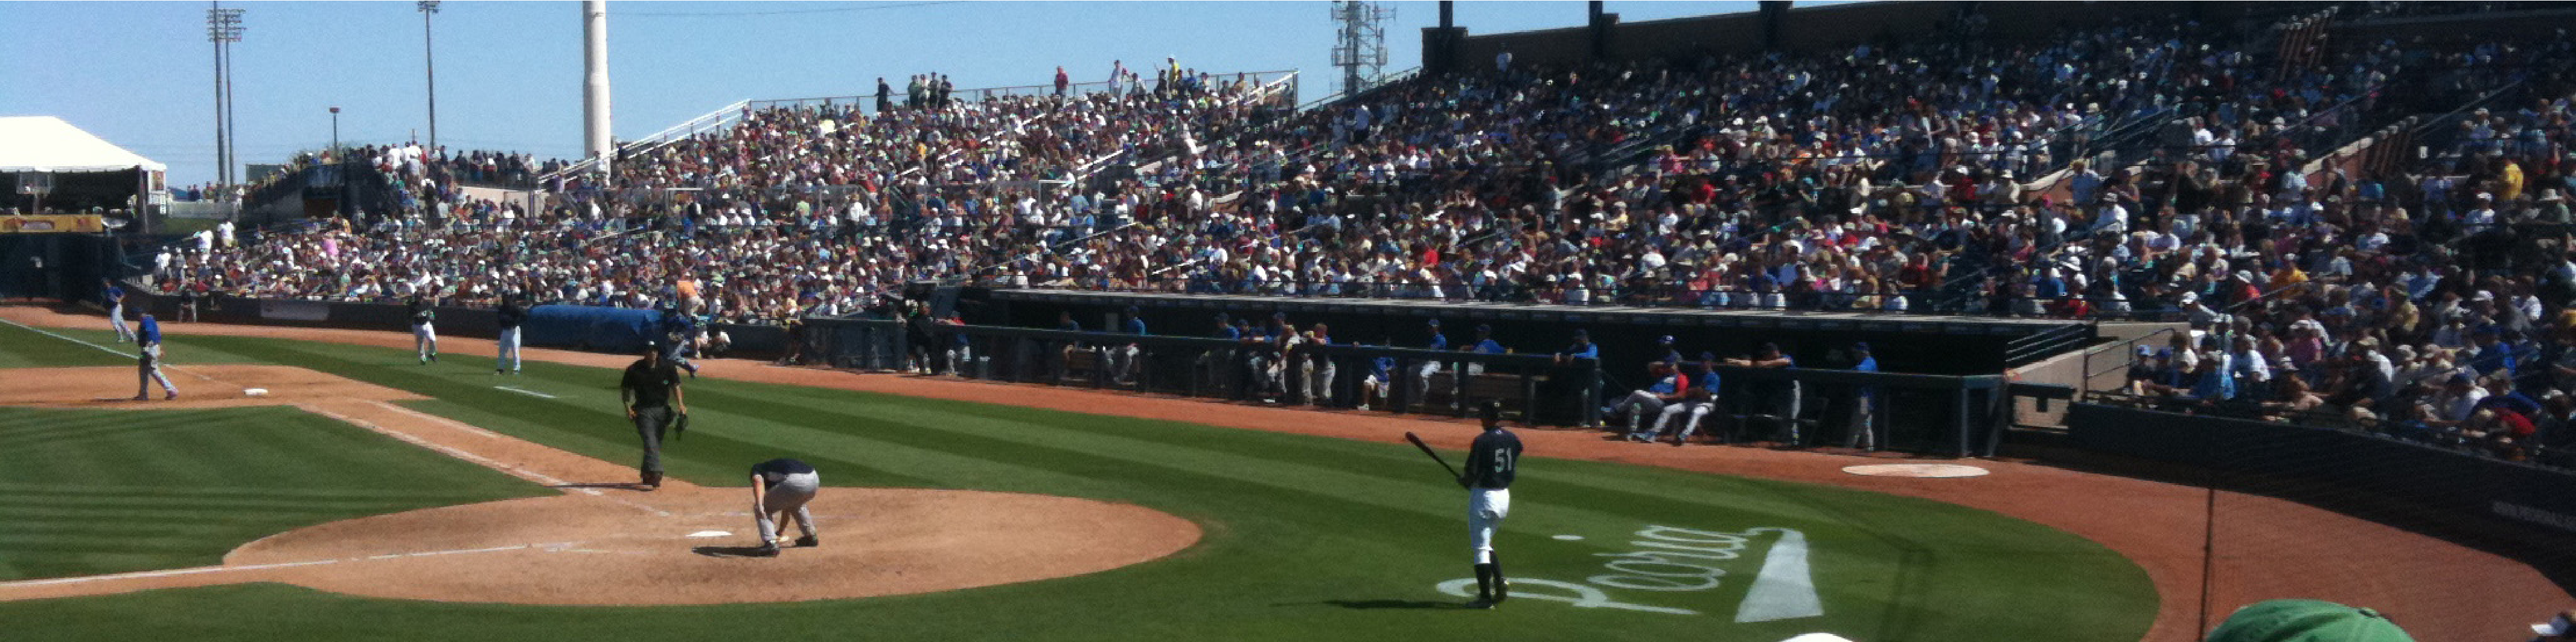
\includegraphics[width=\textwidth]{sampleteaser}
  \caption{Sermeq Kujalleq, Groenlandia, $ITS\_LIVE$ de la NASA.}
  \Description{Imagenes satelitales del Glaciar Sermeq Kujalleq.}
  \label{fig:teaser}
\end{teaserfigure}

\received{20 February 2007}
\received[revised]{12 March 2009}
\received[accepted]{5 June 2009}

%%
%% This command processes the author and affiliation and title
%% information and builds the first part of the formatted document.
\maketitle

\section{Introduction}


La predicción de series de tiempo es una tarea importante en el
ámbito del aprendizaje automático y la ciencia de datos. Desde la
predicción de precios de acciones hasta la predicción del clima, las
series de tiempo son una herramienta valiosa para la toma de decisiones
y la planificación. No obstante, el estudio de series de tiempo en el contexto de los glaciares es un tema menos explorado.

El Ártico se ha calentado hasta cuatro veces más rápido que el resto del planeta durante los últimos 40 años 
y se prevé que las temperaturas globales se calienten aún más en las próximas décadas, 
lo que provocará un importante retroceso de los glaciares durante el siglo XXI \cite{kavan_new_2025}.

Por lo tanto, es crucial comprender, analizar y predecir la velocidad de deshielo de los glaciares para mitigar sus efectos negativos.
En este contexto, la modelación de series de tiempo se convierte en una herramienta esencial para predecir la velocidad de deshielo de los glaciares.
No obstante, para comprender plenamente cómo responden los glaciares al cambio medioambiental 
se necesitarán nuevos métodos que nos ayuden a identificar el inicio de los fenómenos de aceleración del hielo y a observar cómo se propagan las señales dinámicas dentro de los glaciares \cite{greene_detecting_2020}.

En ese sentido, la velocidad de los glaciares es un parámetro importante que nos permite comprender
el comportamiento dinámico de los glaciares y su respuesta al cambio climático \cite{zhang_validation_2024}.
Estudiar la velocidad de los glaciares es crucial para comprender cómo responden al cambio climático y cómo afectan al nivel del mar.

En este trabajo, proponemos un enfoque basado en aprendizaje automático para predecir la serie de tiempo de la velocidad de deshielo de los glaciares.
Utilizamos un conjunto de datos del proyecto  $ITS\_LIVE$ (Time Series of Land Ice Velocity and Elevation) del Jet Propulsion Laboratory de la NASA, que a partir de imágenes satelitales, proporciona información sobre la velocidad de deshielo de los glaciares.
Compararemos los resultados de distintos modelos de aprendizaje automático y discutiremos los resultados obtenidos.

\section{Antecedentes}

A partir de que superar los $1.5\,^\circ\mathrm{C}$ de calentamiento global por encima de los niveles preindustriales se ha convertido en un hecho cada vez más seguro, 
la comunidad científica ha centrado su atención en la preocupación de cambios que esto implica. 
No obstante, todavía no se conocen bien las consecuencias de tal superación de la temperatura global para los glaciares y su contribución al aumento del nivel del mar y a la disponibilidad de agua \cite{schuster_2025}.


Por otro lado, durante la última década el número de observaciones por satélite disponibles ha aumentado considerablemente, 
lo que ha permitido realizar mediciones mucho más frecuentes de la velocidad de los glaciares.
Proyectos como el de Intermission Time Series of Land Ice Velocity and Elevation ($ITS\_LIVE$) de la NASA 
aceleran la comprensión de los procesos críticos de los glaciares y las capas de hielo proporcionando a la comunidad científica registros globales, 
de baja latencia, exhaustivos y de última generación de las velocidades y elevaciones de la superficie observadas desde el espacio \cite{lei_processing_2021} .

Estos datos por lo tanto permiten a través de la modelación de series de tiempo,
predecir la velocidad de los glaciares y su evolución en el tiempo. 

Trabajos como el de Derkacheva et al. \cite{derkacheva_data_2020} han utilizado métodos como Lowess para el estudio de estas series de tiempo, mientras que anteriormente 
ya se habían utlizado modelos de regresión lineal y modelos ARIMA para la predicción de series de tiempo \cite{noauthor_time_2022} sobre otros conjuntos de datos no  $ITS\_LIVE$.

\section{Metodología}

Para la predicción de la velocidad de los glaciares, utilizamos el conjunto de datos del proyecto  $ITS\_LIVE$ de la NASA.
Este conjunto de datos contiene información sobre la velocidad de deshielo de los glaciares a partir de imágenes satelitales.

Cada observación de velocidad de deshielo de los glaciares se registra en un intervalo de tiempo específico, lo que nos permite construir una serie de tiempo.
Para la modelación de series de tiempo, utilizamos distintos modelos de aprendizaje automático, incluyendo modelos de regresión lineal, modelos ARIMA y redes neuronales recurrentes (RNN).

\subsection{Conjunto de Datos}

El conjunto de datos incluye $9$ glaciares y cada uno de estos tiene asociado a un DataFrame con las siguientes variables:

\begin{itemize}
    \item \verb|mid_date|: Fecha media entre las dos imágenes usadas para calcular la velocidad.
    \item \verb|v|: (Variable respuesta) Velocidad total de flujo (magnitud vectorial de vx y vy).
    \item \verb|v_error|:	Error estimado en la velocidad total v.
    \item \verb|vx|:	Componente de velocidad en el eje X (este-oeste).
    \item \verb|vx_error|:	Error en la componente de velocidad vx.
    \item \verb|vy|:	Componente de velocidad en el eje Y (norte-sur).
    \item \verb|vy_error|:	Error en la componente de velocidad vy.
    \item \verb|date_dt|:	Fecha de adquisición como objeto datetime completo.
    \item \verb|satellite_img1|:	Nombre o código del primer satélite usado para la imagen base.
    \item \verb|mission_img1|:	Misión satelital de la primera imagen.
    \item \verb|x|:	Coordenada X en proyección UTM u otra proyección local (EPSG específica).
    \item \verb|y|:	Coordenada Y en proyección UTM u otra.
    \item \verb|lat|:	Latitud geográfica del píxel o punto.
    \item \verb|lon|:	Longitud geográfica del píxel o punto.
    \item \verb|year|:	Año de la observación (extraído de $mid\_date$).
    \item \verb|month|:	Mes de la observación (extraído de $mid\_date$).
    \item \verb|dayofyear|:	Día del año ($1$ a $366$).

\end{itemize}

\subsection{Línea Base}

Para establecer una línea base para la predicción de la velocidad de los glaciares, utilizamos un modelo de regresión lineal simple.
Este modelo se basa en la suposición de que la velocidad de deshielo de los glaciares sigue una tendencia lineal a lo largo del tiempo.
El modelo de regresión lineal se ajusta a los datos de velocidad de deshielo de los glaciares y se utiliza para predecir la velocidad futura.

Además de su simplicidad, la regresión lineal permite interpretar fácilmente la relación entre el tiempo y la velocidad del glaciar mediante sus coeficientes. 
El término de pendiente indica si la velocidad de flujo del glaciar está aumentando o disminuyendo con el tiempo, lo que puede ser un indicio
 de aceleración del deshielo por efectos climáticos. Aunque este modelo no captura patrones estacionales ni fluctuaciones no lineales, sirve como un punto 
 de comparación robusto frente a modelos más complejos como XGBoost o ARIMA, y permite establecer una primera hipótesis sobre la evolución
  temporal del comportamiento glaciar.

\subsection{ARIMA}

El modelo ARIMA (Autoregressive Integrated Moving Average) es un modelo de series de tiempo que combina componentes autorregresivos, de media móvil e integración.
El modelo ARIMA se utiliza para modelar series de tiempo estacionarias y no estacionarias.
Para aplicar el modelo ARIMA a la serie de tiempo de la velocidad de deshielo de los glaciares, primero es necesario transformar la serie de tiempo en una serie estacionaria.
Para ello, se aplican técnicas de diferenciación.

Una vez que se logra la estacionariedad mediante la diferenciación, el modelo ARIMA puede identificar y capturar patrones temporales en la serie, como la dependencia 
entre observaciones pasadas (componente autorregresiva, AR) y los errores de predicción previos (componente de media móvil, MA). En nuestro caso, se ajustó un modelo ARIMA a 
la serie temporal de velocidades de deshielo utilizando la fecha como índice temporal.

\subsection{XGBoost}

XGBoost (Extreme Gradient Boosting) es un algoritmo de aprendizaje automático basado en árboles de decisión que se ha utilizado con éxito en diversas tareas de predicción.
XGBoost es un algoritmo de boosting que combina múltiples árboles de decisión para mejorar la precisión de las predicciones.
Se ha utilizado en diversas aplicaciones, incluida la predicción de series de tiempo.

En el contexto de series de tiempo, aunque XGBoost no modela explícitamente la dependencia temporal como los modelos clásicos (por ejemplo, ARIMA), puede adaptarse para tareas de 
predicción temporal al incorporar variables que representen el tiempo, como el año, mes, día del año o rezagos de la variable objetivo. Su capacidad para capturar relaciones no lineales
 y manejar grandes volúmenes de datos lo convierte en una herramienta eficaz cuando se dispone de múltiples variables explicativas o características derivadas del tiempo. Además, XGBoost
incluye mecanismos de regularización, lo que resulta útil cuando se trabaja con conjuntos de datos ruidosos.


\subsection{LSTM}

Las redes neuronales recurrentes (RNN) son un tipo de modelo de aprendizaje automático que se utiliza para procesar datos secuenciales, como series de tiempo.
Las RNN son capaces de capturar patrones temporales en los datos y se han utilizado con éxito en diversas aplicaciones, incluida la predicción de series de tiempo.
En este trabajo, utilizamos una variante de las RNN llamada LSTM (Long Short-Term Memory), que es especialmente eficaz para modelar dependencias a largo plazo en los datos.

Las redes LSTM superan una de las principales limitaciones de las RNN tradicionales: el problema del desvanecimiento o explosión del gradiente durante el entrenamiento.
 Gracias a su arquitectura con compuertas de entrada, olvido y salida, las LSTM pueden retener información relevante durante períodos más largos y descartar información 
 irrelevante, lo que las hace particularmente adecuadas para modelar series de tiempo con comportamientos complejos o retardos significativos en sus patrones. En este proyecto,
  el modelo LSTM se alimenta con secuencias históricas de velocidad del glaciar para realizar predicciones más precisas del comportamiento futuro.

\subsection{Compración de Resultados}

Para comparar los resultados de los distintos modelos de aprendizaje automático, utilizamos métricas de evaluación que 
describiremos en la siguiente subsección.
Además del desempeño de los modelos, también consideramos la interpretabilidad y la complejidad de cada modelo.
Este análisis comparativo nos permitirá comparar sistemáticamente
el desempeños de los modelos y discutir sus fortalezas y debilidades para este problema en específico.

\subsubsection{Métricas}

Para evaluar el rendimiento de los modelos de aprendizaje automático, utilizamos métricas de evaluación como el error cuadrático medio (MSE) y el coeficiente de determinación (R²).

\begin{itemize}
  \item El error cuadrático medio (MSE) es una métrica que mide la diferencia entre los valores predichos por el modelo y los valores reales de la variable objetivo.
El MSE se calcula como la media de los cuadrados de las diferencias entre los valores predichos y los valores reales.
  \item RMSE es la raíz cuadrada del MSE, lo que nos da una medida de error en las mismas unidades que la variable objetivo.
  Es útil porque nos permite interpretar el error en términos de la variable objetivo y compararlo con los valores reales.
Elegimos el RMSE para este problema en específico porque en el contexto de la predicción de series de tiempo, es importante minimizar los errores grandes para obtener predicciones más precisas.
  \item El coeficiente de determinación (R²) es una métrica que mide la proporción de la varianza de la variable objetivo que es explicada por el modelo.
El R² se calcula como la proporción de la varianza de los valores predichos que es explicada por la varianza de los valores reales.
Es útil porque nos permite evaluar la capacidad del modelo para explicar la variabilidad de los datos.
\end{itemize}

\section{Experimentos y Resultados}

Para evaluar el rendimiento de los modelos de aprendizaje automático, realizamos una serie de experimentos utilizando el conjunto de datos del proyecto  $ITS\_LIVE$ de la NASA.
Seleccionamos un subconjunto de glaciares importantes y obtuvimos las series de tiempo de la velocidad de deshielo de estos glaciares.
El conjunto de datos se dividió en un conjunto de entrenamiento y un conjunto de prueba en un porcentaje de $70\%$ para entrenamiento y $30\%$ para prueba.
Esto debido a que tenemos un mayor cantidad de datos en años reciente en contraste a los primeros años de observación, esto en gran medida debido a la disponibilidad de imágenes satelitales.  
Los modelos se entrenaron utilizando el conjunto de entrenamiento y se evaluaron en el conjunto de prueba.

\subsection{Línea Base}

\paragraph{Estacionalidad}

\begin{figure}[htbp]
   \centering
   \includesvg[width=0.5\textwidth]{svg-inkscape/fft.svg}
    \caption{Transformada de Fourier de la serie de tiempo de la velocidad del glaciar Sermeq Kujalleq en Groenlandia.}
    \label{fig:frequencies}
\end{figure}

En varios de nuestros gráficos, vemos que los datos tienen un elemento estacional. Intuitivamente, sabemos que los datos de la velocidad del glaciar también deberían tener un componente estacional. La velocidad del glaciar debería oscilar cada año, más alta en verano y más baja en invierno. 
Para validar estas sospechas, podemos fijarnos en las transformadas de Fourier de nuestras series.
Las transformadas de Fourier nos permiten convertir una serie basada en la amplitud en una serie basada en la frecuencia. Son funciones de valor complejo que representan cada serie como una superposición de ondas sinusoidales en un plano complejo.

Dado que en la Fig. \ref{fig:frequencies} hay un pico claro cerca de la frecuencia 0.0027 (1/365), eso indica estacionalidad anual.


\paragraph{Estacionariedad}

Una serie temporal es estacionaria cuando sus propiedades estadísticas como la media, la varianza y la autocorrelación no cambian con el tiempo.
Métodos como ARIMA y sus variantes funcionan bajo el supuesto de que la serie temporal que modelizan es estacionaria. Si la serie temporal no es estacionaria, estos métodos no funcionan muy bien.

Utilizamos la prueba de Dickey-Fuller aumentada (ADF) y la prueba de Kwiatkowski-Phillips-Schmidt-Shin (KPSS) para verificar la estacionariedad de nuestras series temporales.
Encontramos que la mayoría de nuestras series temporales no son estacionarias, lo que significa que tienen una tendencia o una varianza que cambia con el tiempo.

Lo que sugiere que modelos como ARIMA y sus variantes no funcionarán bien con nuestras series temporales sin una transformación previa.

\paragraph{OLS}

Para establecer una línea base, utilizamos un modelo de regresión lineal simple (OLS) para predecir la velocidad de los glaciares.

Obtuvimos los siguientes resultados para el modelo OLS

\begin{figure}[htbp]
   \centering
   \includesvg[width=0.5\textwidth]{svg-inkscape/Jakobshavn_OLS_forecast.svg}
    \caption{Predicciones del modelo OLS para el glaciar Jakobshavn.}
    \label{fig:jakobshavn_ols}
\end{figure}

\paragraph{Normalidad de los residuales}

Para verificar la normalidad de los residuales del modelo OLS, utilizamos los siguientes tests.
\begin{itemize}
  \item \textbf{Jarque-Bera}: p-value = $0.0$
  \item \textbf{Shapiro-Wilk}: p-value = $9.27 \times 10^{-40}$
  \item \textbf{Kolmogorov-Smirnov}: p-value = $0.0$
\end{itemize}

Estos resultados indican que los residuales del modelo OLS no siguen una distribución normal, lo que sugiere que el modelo OLS no es adecuado para predecir la velocidad de los glaciares.

\paragraph{Heterocedasticidad}

La heterocedasticidad es un problema común en los modelos de regresión lineal, donde la varianza de los errores no es constante a lo largo de las observaciones.
Para verificar la heterocedasticidad de los residuales del modelo OLS, utilizamos los siguientes tests.

\begin{itemize}
  \item \textbf{Breusch–Pagan}: p-value = $6.58 \times 10^{-5}$
  \item \textbf{White}: p-value = $4.69 \times 10^{-8}$
\end{itemize}

Estos resultados indican que los residuales del modelo OLS presentan heterocedasticidad, lo que significa que la varianza de los errores no es constante a lo largo de las observaciones.

\paragraph{Resultados del modelo OLS}

Los resultados del modelo OLS se muestran en la Figura \ref{fig:jakobshavn_ols} y en la Tabla \ref{tab:ols}.

\begin{table}[H]
  \caption{Resultados del modelo OLS}
  \label{tab:ols}
  \begin{tabular}{lc}
    \toprule
    Métrica & Valor \\
    \midrule
    MA & 1698.99 \\
    MSE & 3\,468\,429.84 \\
    RMSE & 1\,862.37 \\
    $R^2$ & 0.400 \\
    Adj. $R^2$ & 0.399 \\
    \bottomrule
  \end{tabular}
\end{table}

A pesar de que el modelo OLS tiene un $R^2$ de $0.4$, lo que indica que el modelo explica el $40\%$ de la varianza de los datos,
los resultados no son muy buenos, ya que el RMSE es de $1862.37$, lo que indica que el modelo tiene un error cuadrático medio alto.
Esperábamos que el modelo OLS no funcionara muy bien debido a los criterios de estacionariedad y normalidad que revisamos anteriormente.
No ostante, el modelo OLS sirve como una línea base para comparar los resultados de los otros modelos de aprendizaje automático.
Adicionalmente podemos observar una tendencia creciente en la serie temporal, lo que indica que la velocidad de los glaciares está aumentando con el tiempo.

\subsection{ARIMA}

A continuación se presenta la gráfica obtenida al aplicar un modelo $ARIMA(p=9,d=1,q=2)$ cuyos parámetros representan
\begin{itemize}
  \item \verb|p|: Número de retardos autorregresivos (AR).
  \item \verb|d|: Número de diferencias necesarias para hacer la serie estacionaria.
  \item \verb|q|: Número de términos de media móvil (MA)
\end{itemize}

a los datos del glaciar Alaska-Columbia Glacier

\begin{figure}[H]
    \centering
    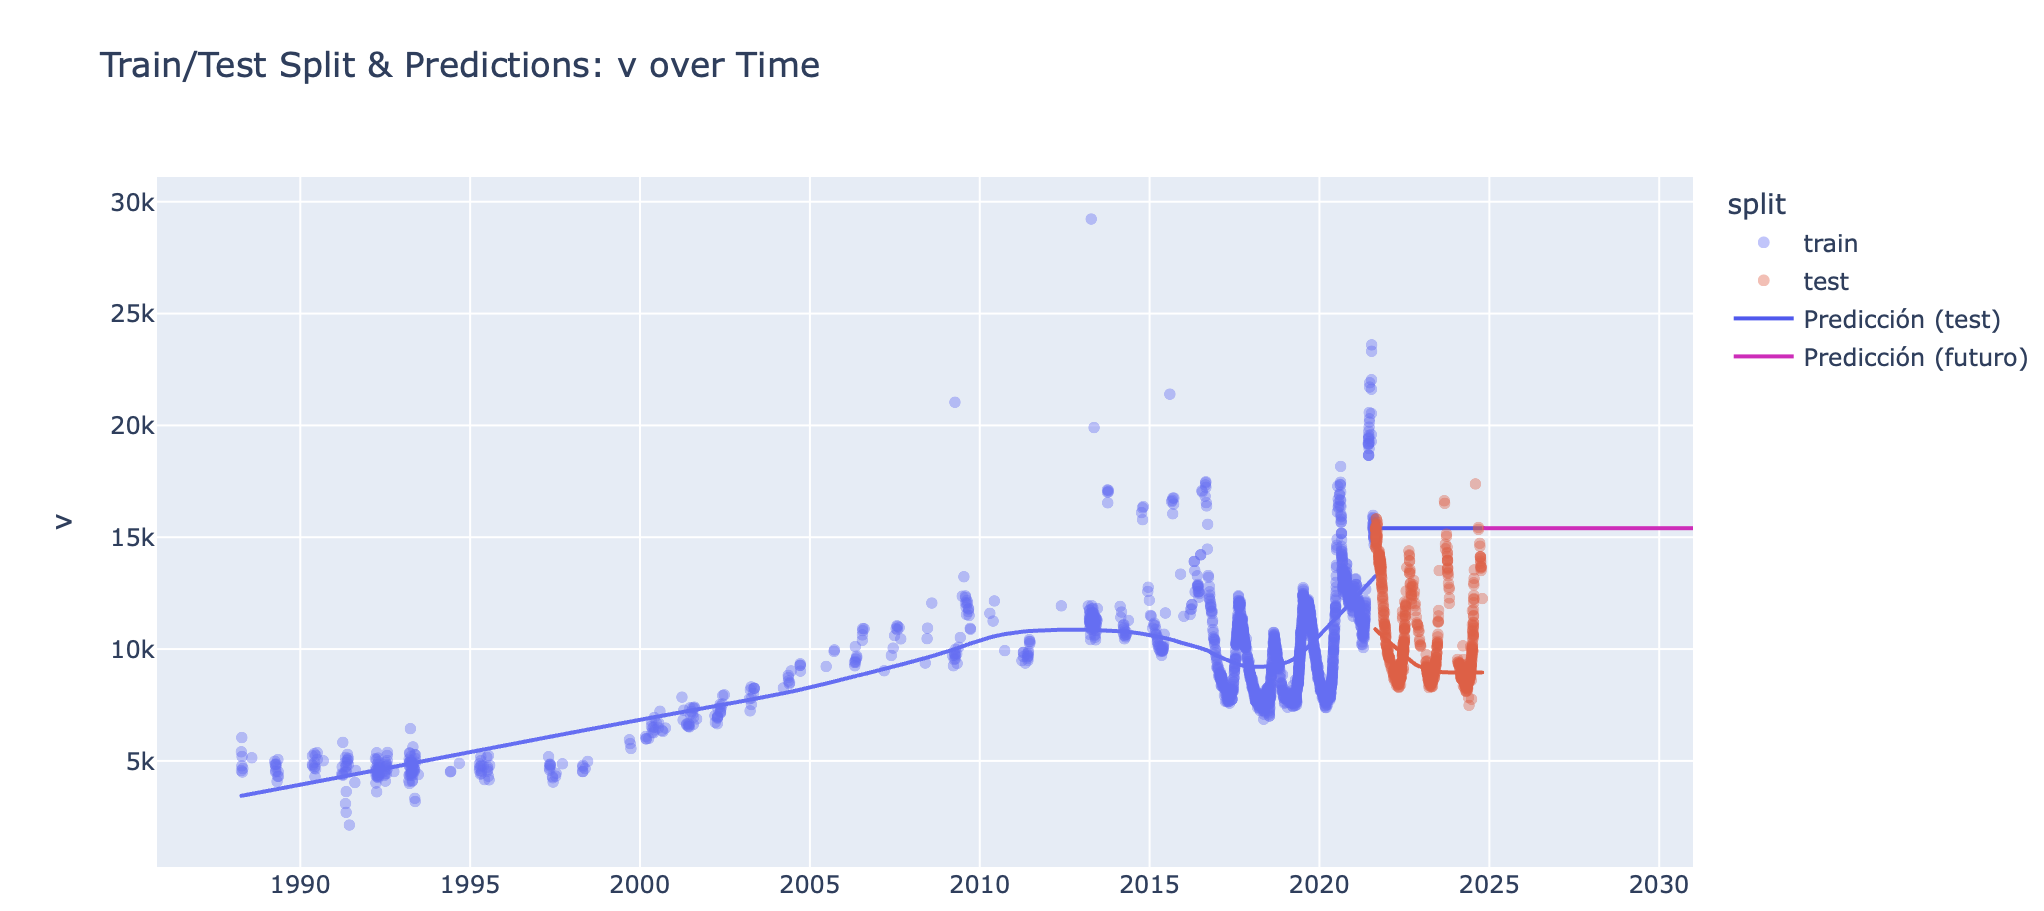
\includegraphics[width=0.5\textwidth]{ARIMA1.png} % o {images/glaciar.png} si está en subcarpeta
    \caption{Predicciones del modelo ARIMA para el glaciar Jakobshavn}
    \label{fig:ARIMA1}
\end{figure}

Podemos observar que la serie parece tener ciclos anuales o multianuales bien definidos sin embargo el modelo
no sigue del todo estas oscilaciones, indicando que el modelo tiene limitaciones para capturar esta estacionalidad. 
Esto lo podemos ver en la línea azul que representa las predicciones en el conjunto de prueba.

Por otro lado las predicciones a futuro que realiza el modelo son constantes, lo que significa que 

\begin{itemize}
  \item El modelo ya no tiene nueva estructura que extrapolar.
  \item Asume que la última tendencia o nivel es estacionario.
\end{itemize}

A continuación se muestra una tabla con las métricas de evaluación del modelo

\begin{table}[H]
  \caption{Resultados del modelo ARIMA}
  \label{tab:ARIMA}
  \begin{tabular}{lc}
    \toprule
    Métrica & Valor \\
    \midrule
    MAE & 5,416.85 \\
    MSE & 3,293,357 \\
    RMSE & 5,738.77 \\
    $R^2$ & -0.788 \\
    Adj. $R^2$ & -0.796 \\
    \bottomrule
  \end{tabular}
\end{table}

El modelo ARIMA mostró limitaciones importantes debido a la naturaleza no estacionaria y estacional de la serie de tiempo
ya que realiza un trabajo de ajuste y predicción muy malo, que se traduce en un MSE es muy alto, debido además a la presencia de ruido satelital (outliers),
además el $R^{2}$ negativo indica que  el modelo predice mucho peor que seleccionar el valor medio de los datos.

A pesar de aplicar una diferenciación de orden uno, los resultados sugieren  que la serie aún no era estacionaria, lo cual compromete la validez de los supuestos
 de ARIMA. Además, la estacionalidad  no pudo ser capturada adecuadamente por un modelo ARIMA estándar, lo que resultó en predicciones planas y métricas
 de desempeño pobres (R² < 0).

\subsection{XGBoost}

Para el modelo XGBoost, tuvimos que utilizar características adicionales.
Estas características incluyen el año, mes, día del año, lags, rolling windows y diferencias de la variable objetivo.
Adicionalmente, utilizamos GridSearchCV de Scikit-learn \cite{Pedregosa_Scikit-learn_Machine_Learning_2011} para encontrar los mejores hiperparámetros del modelo XGBoost los cuales se muestran en la Tabla \ref{tab:xgb_params}.

\begin{table}[H]
  %Mejores parametros
  \caption{Mejores hiperparámetros del modelo XGBoost}
  \label{tab:xgb_params}
  \begin{tabular}{lc}
    \toprule
    Hiperparámetro & Valor \\
    \midrule
    colsample\_bytree & 0.7 \\
    learning\_rate & 0.1 \\
    max\_depth & 3 \\
    n\_estimators & 1000 \\
    subsample & 0.7 \\
    \bottomrule
  \end{tabular}
\end{table}

Los resultados obtenidos con el modelo que se muestra en la Figura \ref{fig:jakobshavn_xgb}
son bastante buenos, ya que el modelo logra capturar la estacionalidad de la serie de tiempo y las predicciones son más precisas que las del modelo OLS y ARIMA.
No obstante, para predicciones futuras fuera del rango de datos de entrenamiento, el modelo XGBoost no extrapola bien.
Esto en mayor medida debido a que el modelo no captura la estructura temporal de la serie de tiempo, sino que se basa en las características adicionales que le proporcionamos.

\begin{table}[H]
  \caption{Resultados del modelo XGBoost}
  \label{tab:xgb}
  \begin{tabular}{lc}
    \toprule
    Métrica & Valor \\
    \midrule
    MAE & 112.34 \\
    MSE & 177600.20 \\
    RMSE & 421.43 \\
    $R^2$ & 0.9547 \\
    Adj. $R^2$ & 0.9546 \\
    \bottomrule
  \end{tabular}
\end{table}

\begin{figure}[htbp]
   \centering
   \includesvg[width=0.5\textwidth]{svg-inkscape/Jakobshavn_XGB_forecast.svg}
    \caption{Predicciones del modelo XGBoost para el glaciar Jakobshavn.}
    \label{fig:jakobshavn_xgb}
\end{figure}


\subsection{LSTM}

Para el modelo LSTM, utilizamos una arquitectura de red neuronal recurrente con capas LSTM.
El modelo LSTM utilizado consiste en dos capas LSTM bidireccionales con 64 unidades ocultas, seguidas de una capa densa y con un total de 145537 parámetros. 
El modelo fue implementado utilizando Pytorch \cite{Ansel_PyTorch_2_Faster_2024} y se entrenó durante 30 épocas usando el optimizador Adam y la función de pérdida MSE, aplicando scheduled sampling para mejorar la generalización.
Para la preparación de los datos de entrenamiento, se generaron características adicionales a partir de las columnas de fecha y la variable objetivo, como rezagos (lags), medias móviles y codificación estacional con funciones seno y coseno del día del año. Posteriormente, los datos se dividieron en conjuntos de entrenamiento y prueba (70\% y 30\% respectivamente).
Además los datos se normalizaron utilizando el StandardScaler de Scikit-learn para que las características tuvieran media cero y desviación estándar uno, lo que es crucial para el buen funcionamiento de las redes neuronales.
Finalmente, se transformaron en secuencias para alimentar el modelo LSTM, permitiendo capturar dependencias temporales y patrones estacionales en la serie de tiempo.
Esto es especialmente importante en las redes LSTM, ya que están diseñadas para manejar datos secuenciales y aprender de las relaciones temporales en los datos.


\begin{figure}[htbp]
   \centering
   \includesvg[width=0.5\textwidth]{svg-inkscape/Jakobshavn_LSTM_forecast.svg}
    \caption{Predicciones del modelo LSTM para el glaciar Jakobshavn.}
    \label{fig:jakobshavn_lstm}
\end{figure}

Obtuvimos buenos resultados con el modelo LSTM, ya que el modelo logra capturar la estacionalidad de la serie de tiempo y las predicciones son más precisas que las del modelo OLS y ARIMA.
No obstante, al igual que con el modelo XGBoost, el modelo LSTM no extrapola bien para predicciones futuras fuera del rango de datos de entrenamiento. 
Sin embargo el modelo LSTM logra capturar la estructura temporal de la serie de tiempo y la tendencia de aumento 
de la velocidad de deshielo de los glaciares.

\begin{table}[H]
  \caption{Resultados del modelo LSTM}
  \label{tab:lstm}
  \begin{tabular}{lc}
    \toprule
    Métrica & Valor \\
    \midrule
    MAE & 218.40 \\
    MSE & 136648.44 \\
    RMSE & 369.66 \\
    $R^2$ & 0.9625 \\
    Adj. $R^2$ & 0.9622 \\
    \bottomrule
  \end{tabular}
\end{table}

\subsection{Discusión}

Los resultados obtenidos con los distintos modelos de aprendizaje automático muestran que los modelos de aprendizaje automático son capaces de capturar la estacionalidad y la tendencia de aumento de la velocidad de deshielo de los glaciares.
El modelo OLS, aunque simple, sirve como una línea base y muestra que la velocidad de deshielo de los glaciares tiene una tendencia creciente.
El modelo ARIMA, aunque conceptualmente apropiado para datos temporales, no logró capturar adecuadamente la estructura estacional de los glaciares y sus predicciones fueron planas, lo que sugiere que su aplicabilidad directa es limitada para series con estacionalidad y ruido como las de  $ITS\_LIVE$.
El modelo XGBoost demostró gran capacidad predictiva al incorporar variables derivadas del tiempo (lags, rolling, mes, año, etc.), lo que compensó su incapacidad nativa para modelar secuencias.
El modelo LSTM, al aprovechar su arquitectura de memoria, fue el modelo más preciso, mostrando gran potencial para modelar dependencias de largo plazo en los glaciares.
Es importante notar que a pesar de que utilizar features adicionales, esto implica que las predicciones futuras (a manera autorregresiva) no son extrapolables.

Se trata de un problema complejo, ya que la velocidad de deshielo de los glaciares es un fenómeno natural que está influenciado por muchos factores, como el clima, la topografía y la geología.
Los datos que utilizamos son limitados y no contienen toda la información necesaria para predecir la velocidad de deshielo de los glaciares mas allá de la temporalidad.
Este trabajo podria ser indudablemente mejorado con la incorporación de datos adicionales como datos climáticos. 
No obstante, los resultados son satisfactorios ya que muestran que los modelos de aprendizaje automatico pueden ser útiles para esta tarea.

\section{Conclusiones}

En este trabajo, hemos propuesto un enfoque basado en aprendizaje automático para predecir la serie de tiempo de la velocidad de deshielo de los glaciares, permitiendonos concluir para
cada modelo lo siguiente:
\begin{itemize}
  \item La regresión lineal (OLS) mostró una capacidad limitada de ajuste, pero su simplicidad permite una interpretación directa de tendencias, sirviendo como línea base.
  \item El modelo ARIMA, si bien conceptualmente apropiado para datos temporales, no logró capturar adecuadamente la estructura estacional de los glaciares. Las métricas de 
desempeño ($R^2$ negativo) y las predicciones planas sugieren que su aplicabilidad directa es limitada para series con estacionalidad y ruido como las de ITS\_LIVE.
  \item XGBoost demostró gran capacidad predictiva ($R^2 \approx 0.95$) al incorporar variables derivadas del tiempo (lags, rolling, mes, año, etc.), lo que compensó su incapacidad nativa para modelar secuencias.
  \item LSTM, al aprovechar su arquitectura de memoria, fue el modelo más preciso ($R^{2} > 0.96$), mostrando gran potencial para modelar dependencias de largo plazo en los glaciares.

  \end{itemize}
Encontramos que los modelos de aprendizaje automático, son herramientas valiosas para la predicción de series de tiempo en el contexto de los glaciares ya que los resultados obtenidos muestran que estos  
pueden capturar patrones temporales en la velocidad de deshielo de los glaciares y proporcionar predicciones precisas.

En resumen, los resultados sugieren que los modelos de aprendizaje automático superan significativamente a los modelos clásicos en esta tarea, especialmente cuando se combinan con un buen diseño de variables y preprocesamiento. 
Para futuros experimentos  se podrían explorar modelos híbridos (SARIMA-LSTM, DeepAR) y aplicar explicabilidad (SHAP, LRP) para entender las contribuciones temporales y estacionales a la predicción.

\section{Appendices}
%%
%% The acknowledgments section is defined using the "acks" environment
%% (and NOT an unnumbered section). This ensures the proper
%% identification of the section in the article metadata, and the
%% consistent spelling of the heading.
\begin{acks}
Agradecemos a la clase de la Maestría en Ciencias e Ingenierías de la Computación de la UNAM por su apoyo y orientación en este trabajo.
Agradecemos al Jet Propulsion Laboratory de la NASA por proporcionar el conjunto de datos del proyecto  $ITS\_LIVE$.
\end{acks}

%%
%% The next two lines define the bibliography style to be used, and
%% the bibliography file.
\bibliographystyle{ACM-Reference-Format}
\bibliography{sample-base}

%%
%% If your work has an appendix, this is the place to put it.
\appendix

\end{document}
\endinput
%%
%% End of file `sample-sigconf-authordraft.tex'.
